\section{Mô phỏng mạch trên PSpice}
\subsection{Mạch 3.3V regulator}
Đầu tiên, chúng ta sẽ sử dụng đầu vào là nguồn DC 20 V để kiểm thử đầu ra.

\begin{figure}[ht]
    \centering
    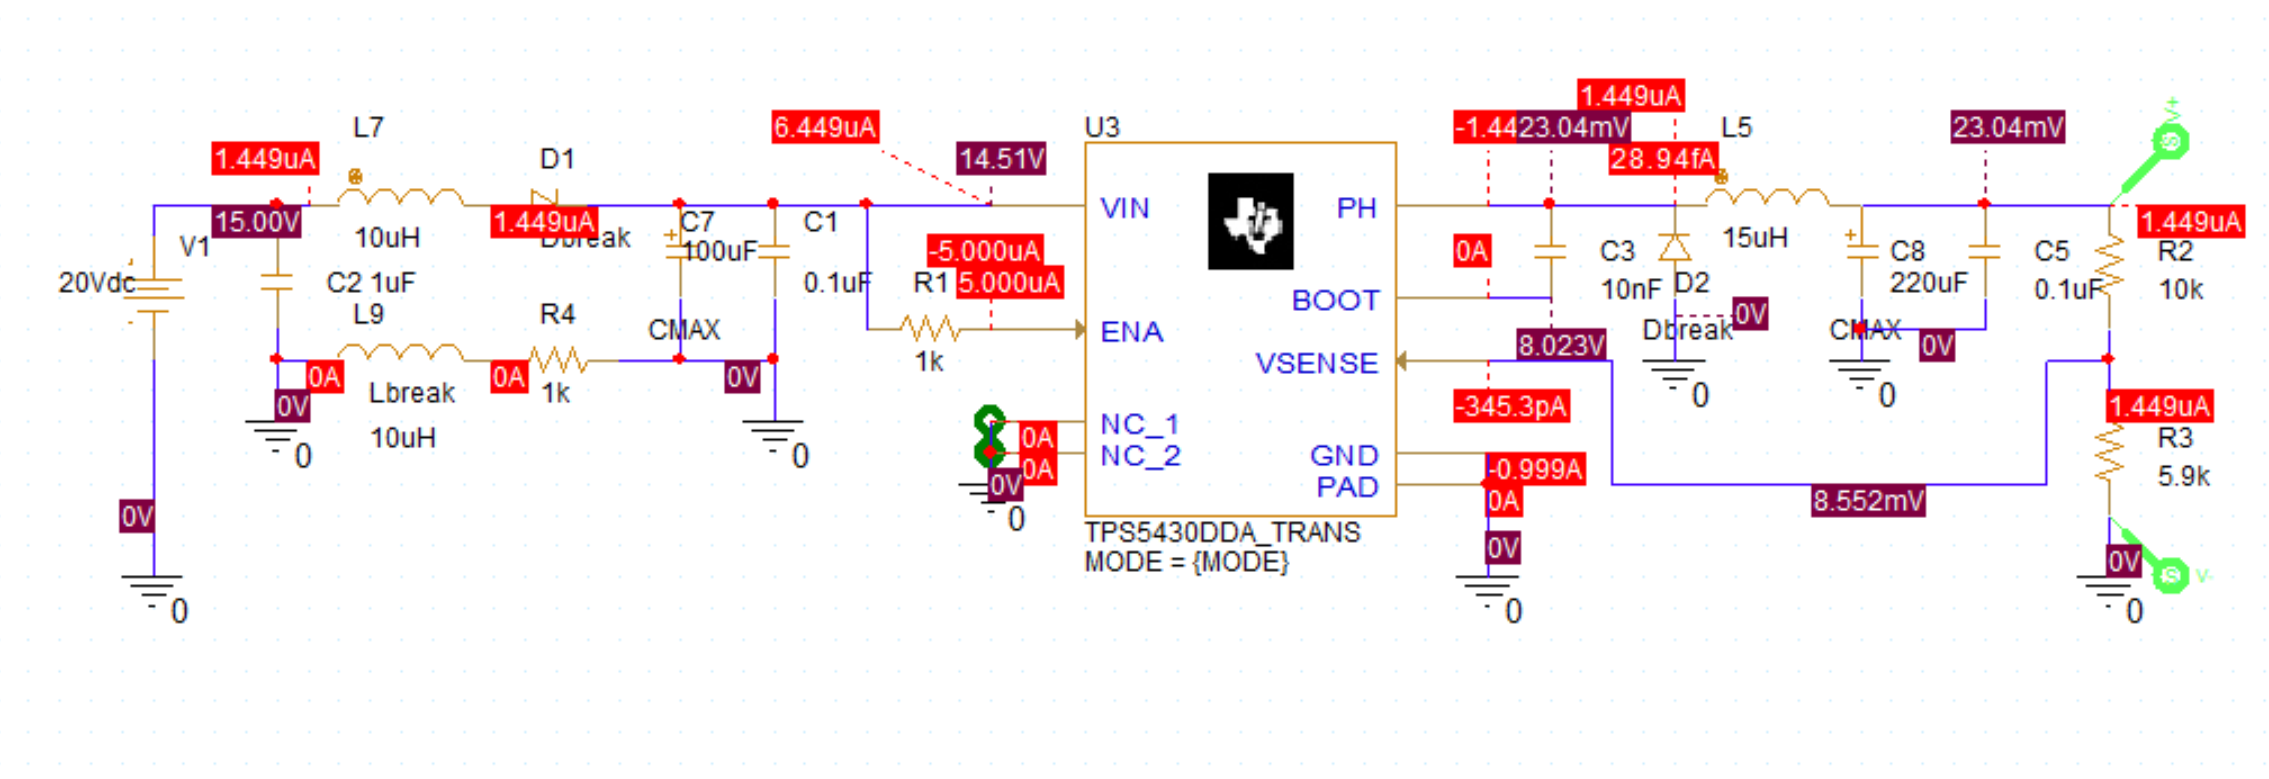
\includegraphics[width=1\textwidth]{graphics/section4/f1.png}
    \caption{Nguồn DC 20 V}
\end{figure}

\textbf{Ảnh mô phỏng}
\begin{figure}[ht]
    \centering
    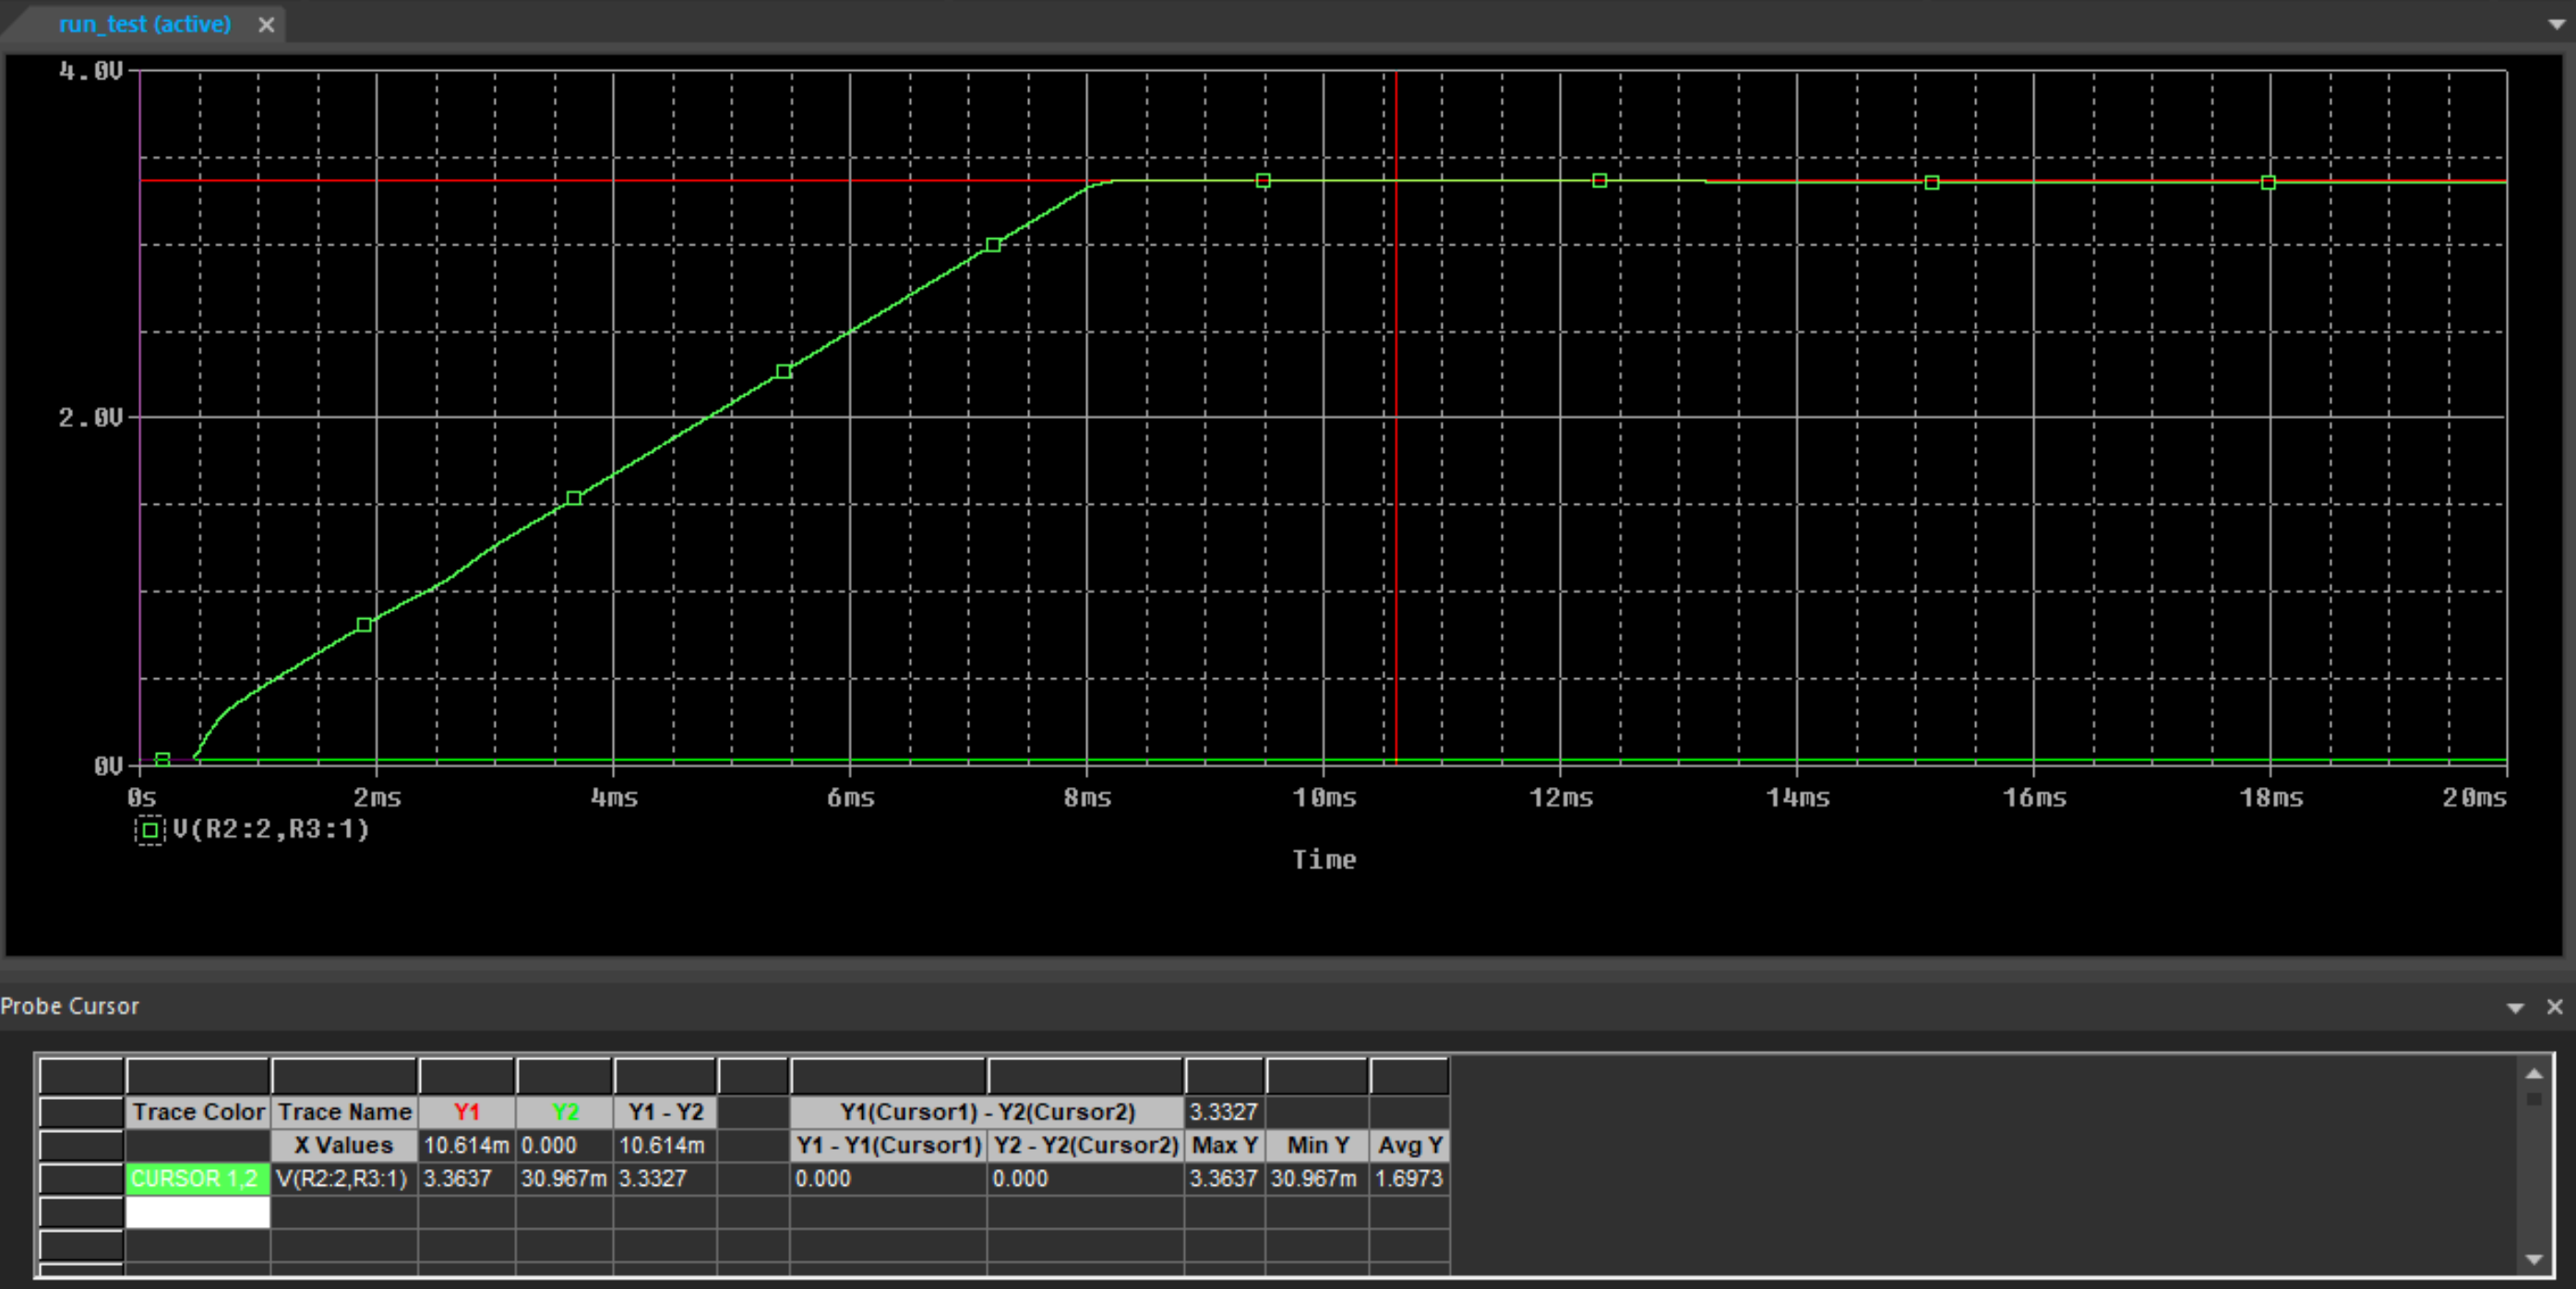
\includegraphics[width=1\textwidth]{graphics/section4/f2.png}
    \caption{Nguồn DC 20 V}
\end{figure}

\textbf{Nhận xét: }Nguồn đầu vào 20 V DC khi qua mạch cho đầu ra ổn định ở mức 3.3V DC. Như vậy, mạch đã hoạt động đúng như yêu cầu.

Tiếp theo ta sẽ cho nguồn đầu vào là tín hiệu AC được dùng như nguồn nhiễu với điện áp gốc (VDC) là 15V và tín hiệu nhiệu (VAC) là 6V.

\begin{figure}[ht]
    \centering
    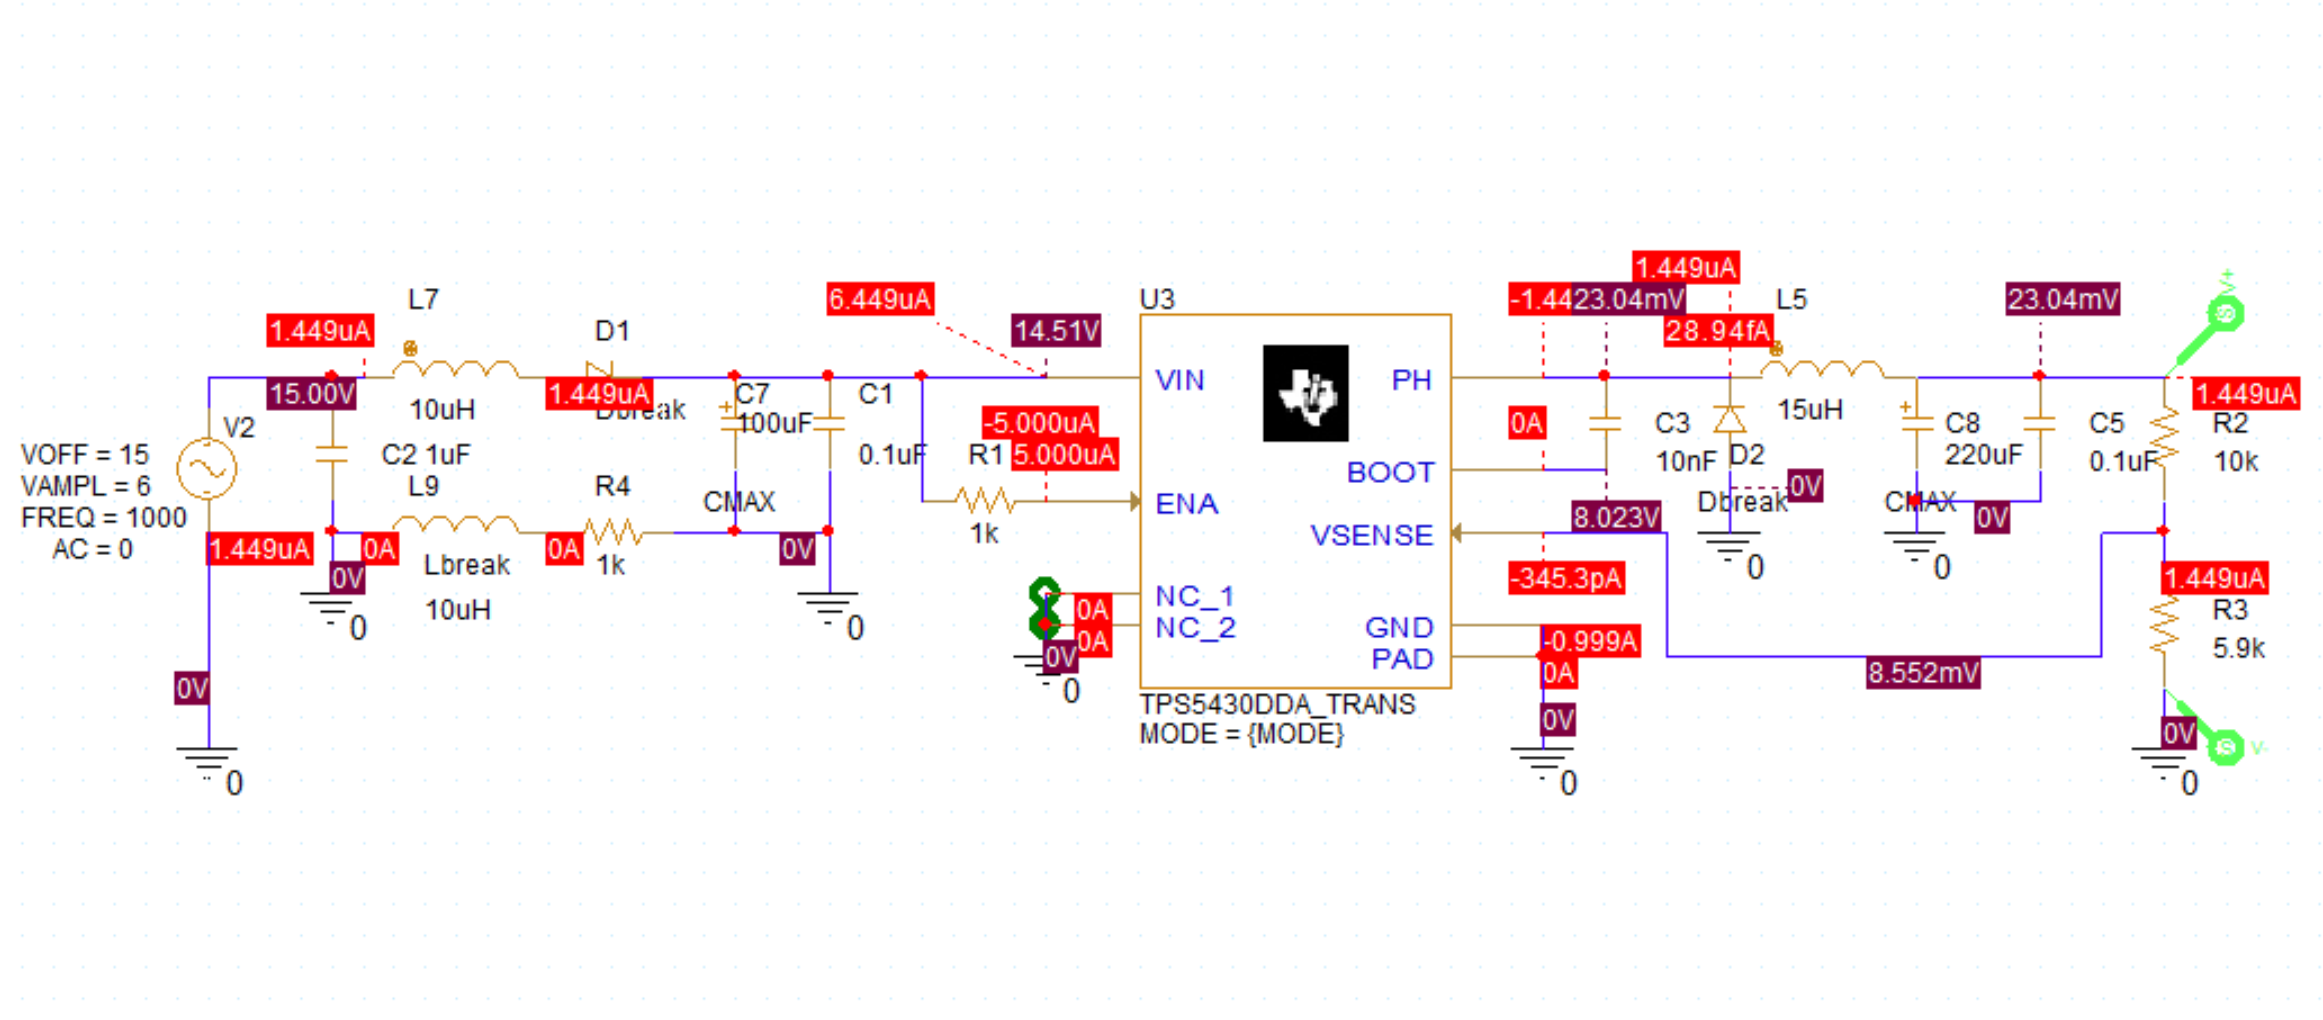
\includegraphics[width=1\textwidth]{graphics/section4/f3.png}
    \caption{Nguồn nhiễu}
\end{figure}

\textbf{Ảnh mô phỏng}
\begin{figure}[ht]
    \centering
    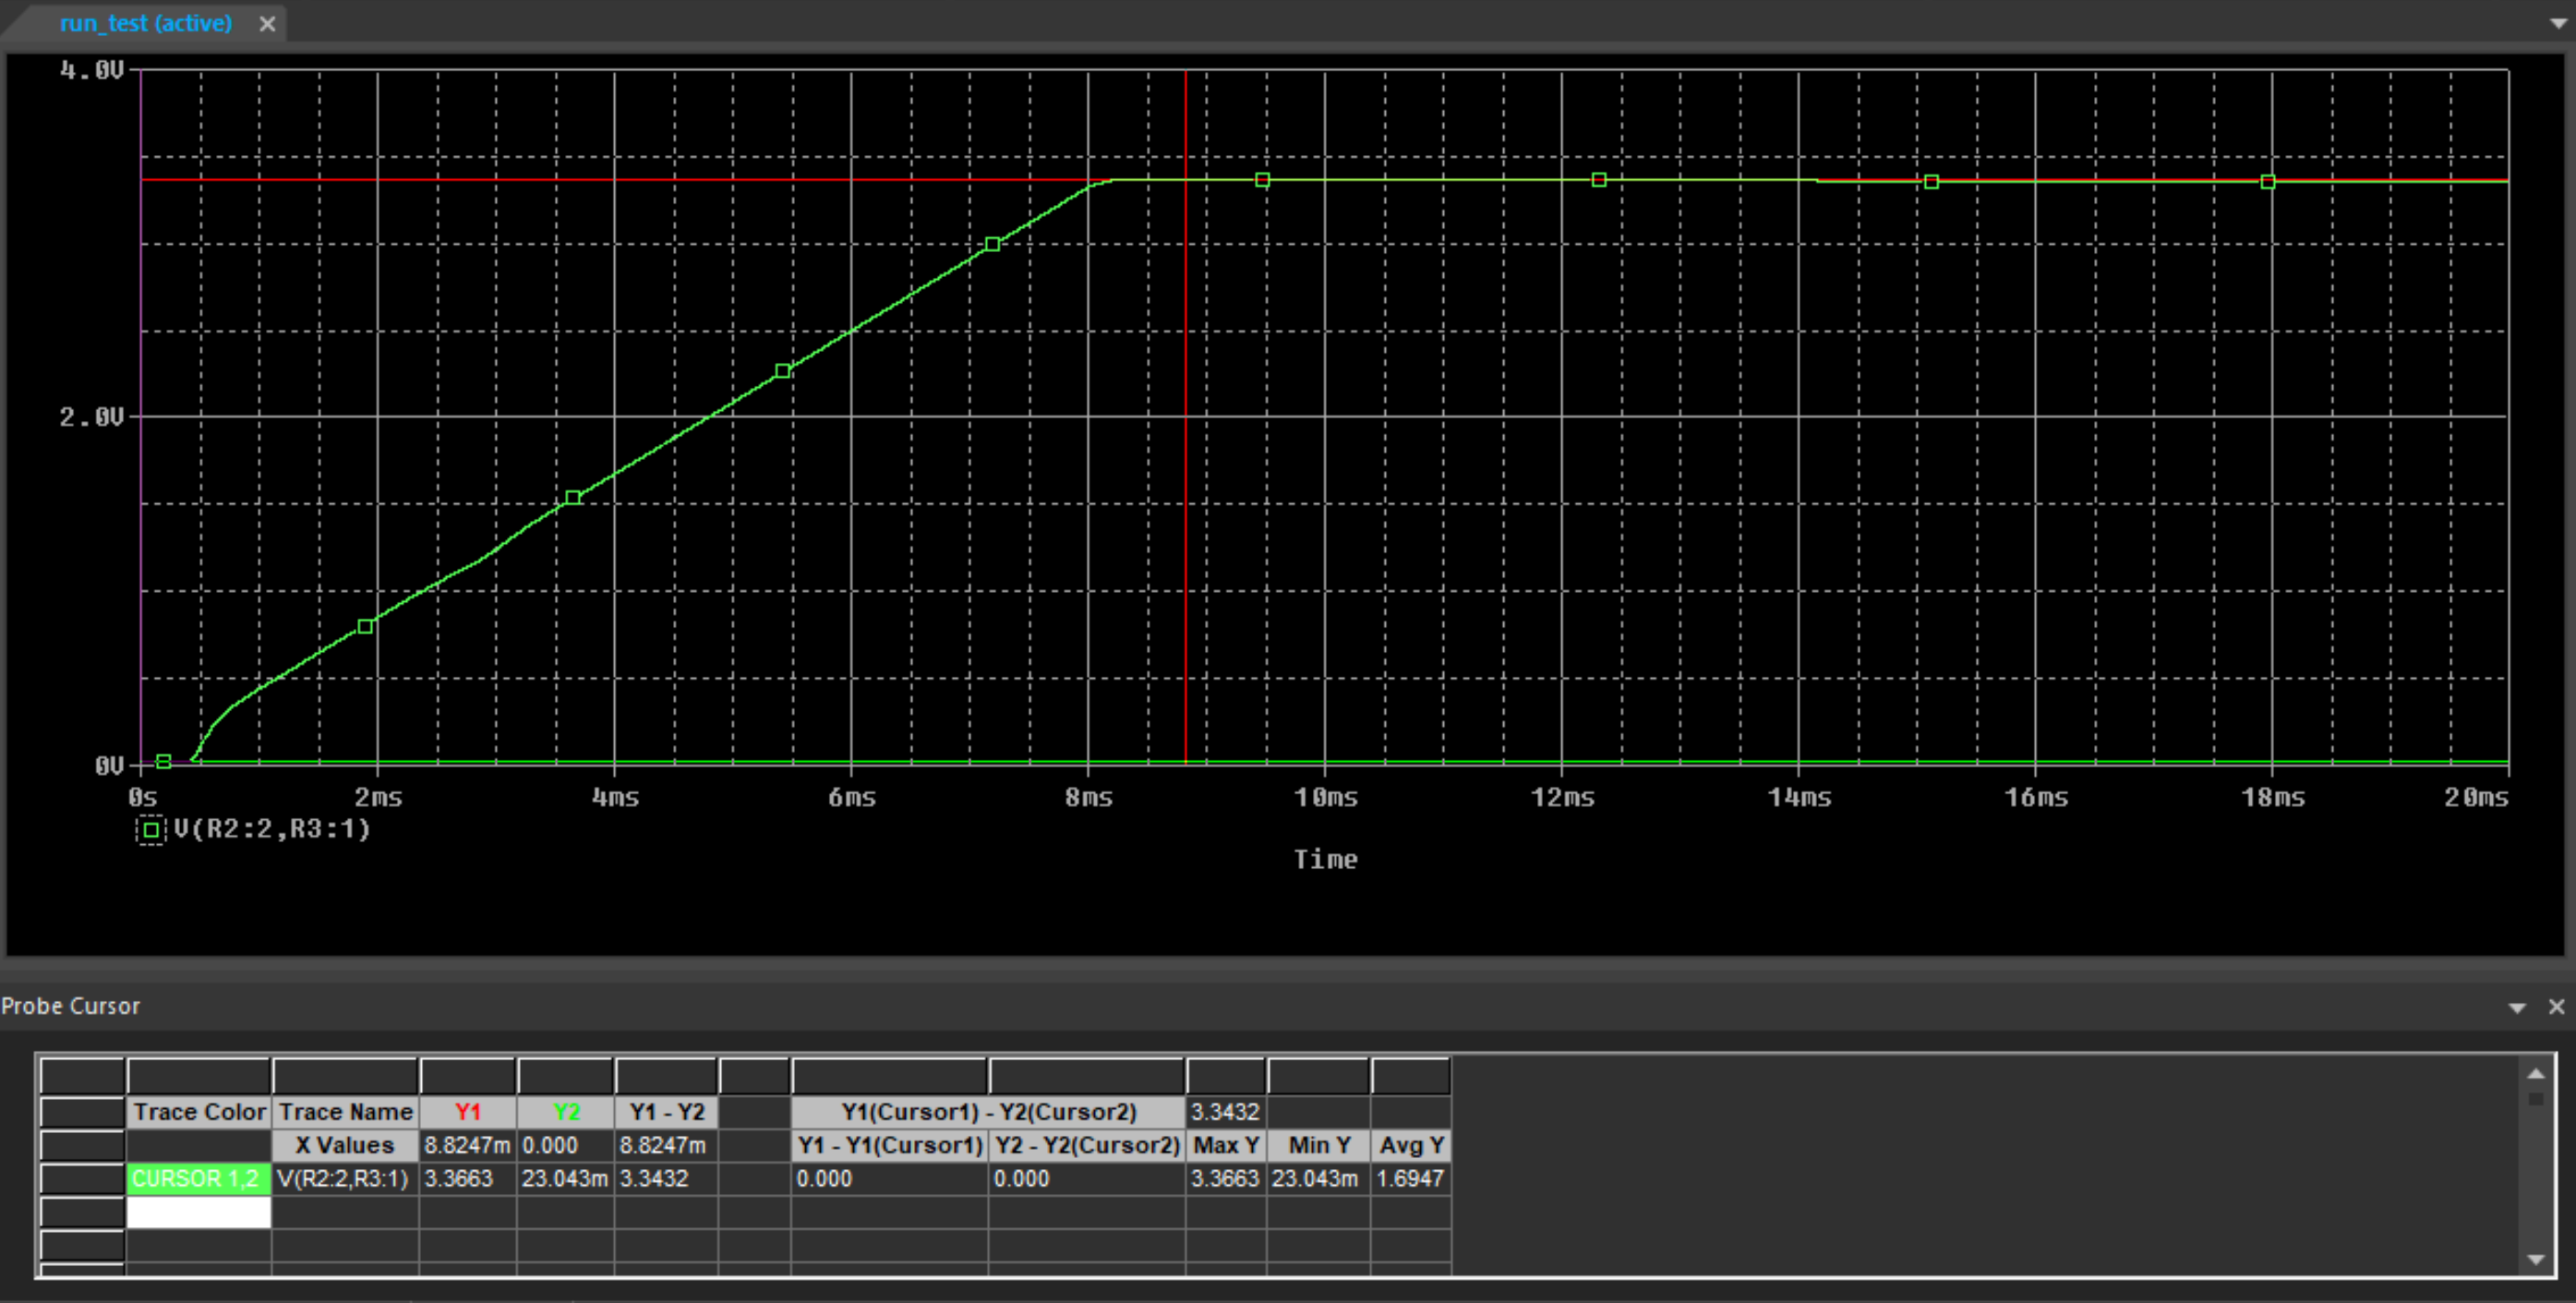
\includegraphics[width=0.95\textwidth]{graphics/section4/f4.png}
    \caption{Nguồn DC 20 V}
\end{figure}

\textbf{Nhận xét: }Mạch đã lọc và giảm áp ổn định ở mức 3.3 V. Như vậy mạch nguồn cần kiểm tra thỏa yêu cầu chức năng.
\pagebreak
\subsection{Current sensor circuit}
Current sensor TA12 và TA17 là những cảm biến để đo tín hiệu AC có dòng tối đa 5A với TA12 và dòng tối đa 10A với TA17. Đầu ra của 2 tín hiệu là tín hiệu AC có cùng tần số với dòng đang đo và biên độ nhỏ hơn.

Trong schematic của TA12 (hoặc TA17), ta thấy dòng đầu ra AC max là 0.5mA nên ta sẽ dùng 1 nguồn điện AC với biên độ khoảng 0.5mA để xem thử khi mạch hoạt động thế nào khi đó dòng điện.

\textbf{Mô phỏng}

\begin{figure}[ht]
    \centering
    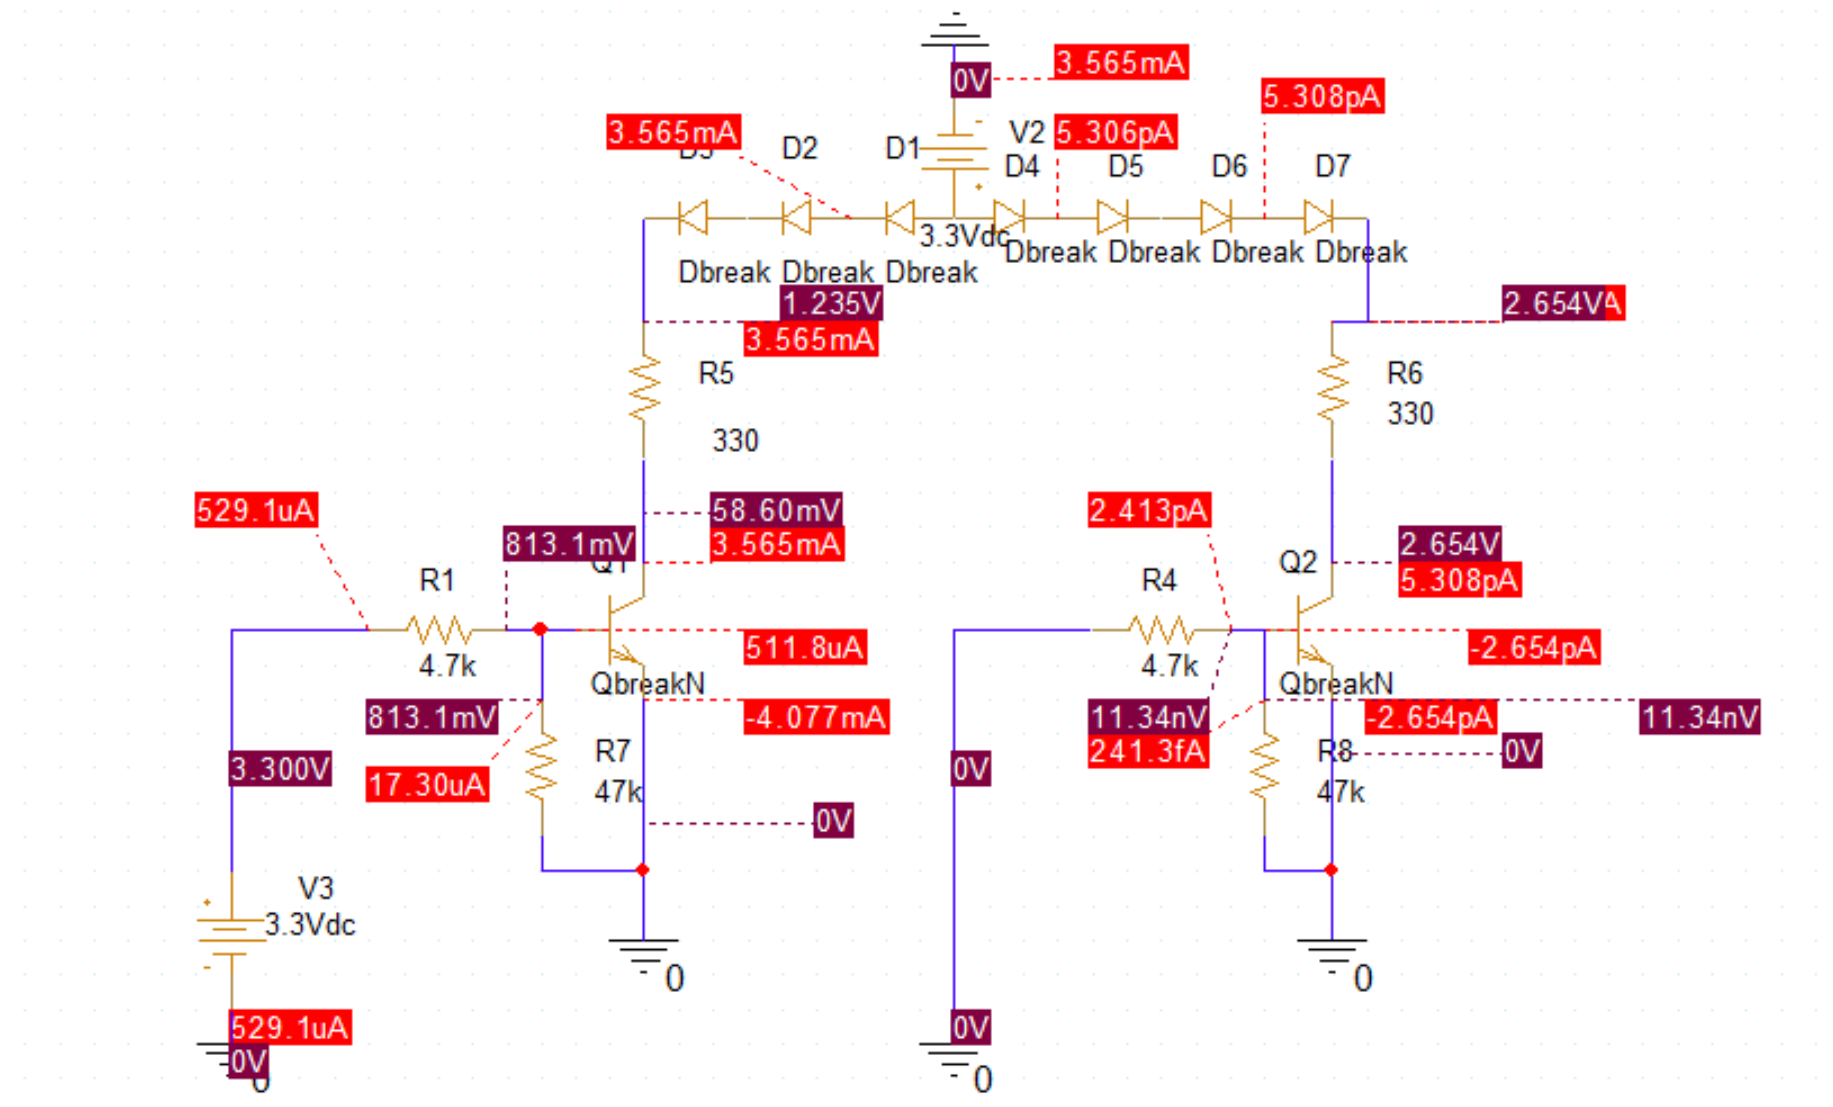
\includegraphics[width=0.95\textwidth]{graphics/section4/f6.png}
    \caption{Nguồn AC 0.5mA}
\end{figure}

\begin{figure}[ht]
    \centering
    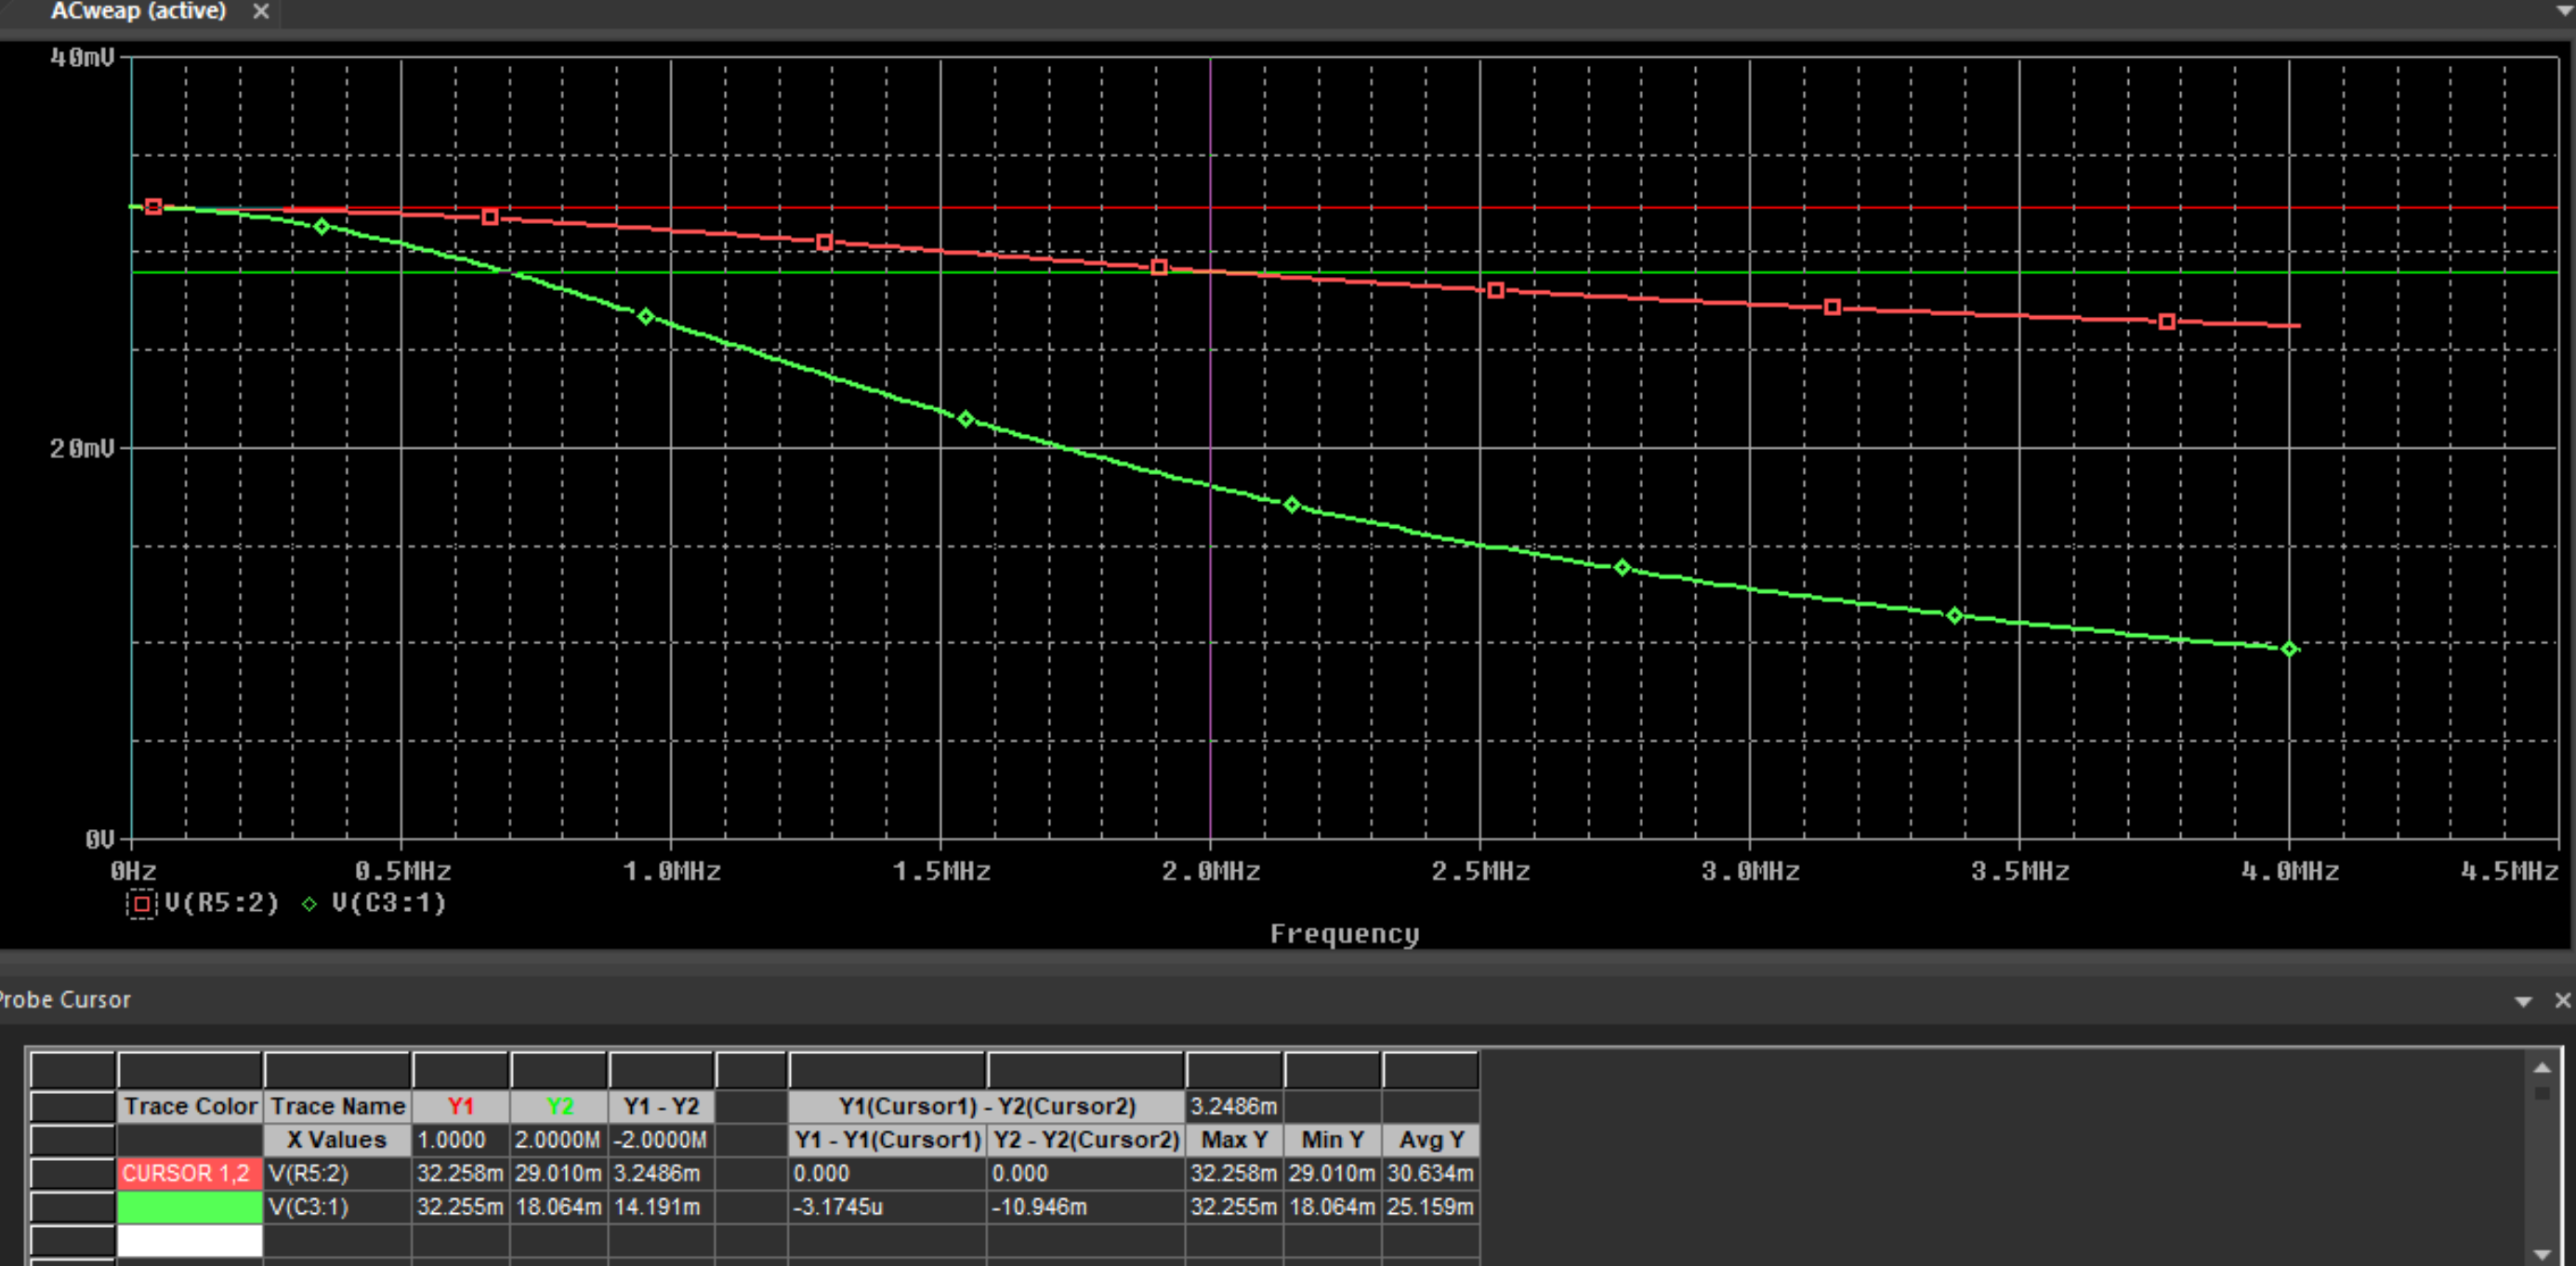
\includegraphics[width=0.95\textwidth]{graphics/section4/f7.png}
    \caption{Nguồn AC 0.5mA thay đổi tần số từ 1Hz đến 4Mhz}
\end{figure}

\textbf{Nhận xét:} Ta thấy đầu ra của ADC\_CH6 được opamp khếch đại lên Gain = 2 khi tần số rất thấp và giảm dần khi tần số tăng. Điều này cho thấy mạch lọc thông thấp đang hoạt động.

\pagebreak
\subsection{Interface with high-current LEDs}
Do điện áp phân cực thuận $V_{f_{RED}} = 1.8V$ tới 2.2V và trong mô phỏng trên PSpice thì $V_F \approx 0.67 V$ nên ta thay bằng 3 diode.
Tương tự, $V_{f_{GREEN}} = 2.8V$ tới 3.2V nên trong mô phỏng ta thay bằng 4 diode.

\textbf{Ảnh mô phỏng}

\begin{figure}[ht]
    \centering
    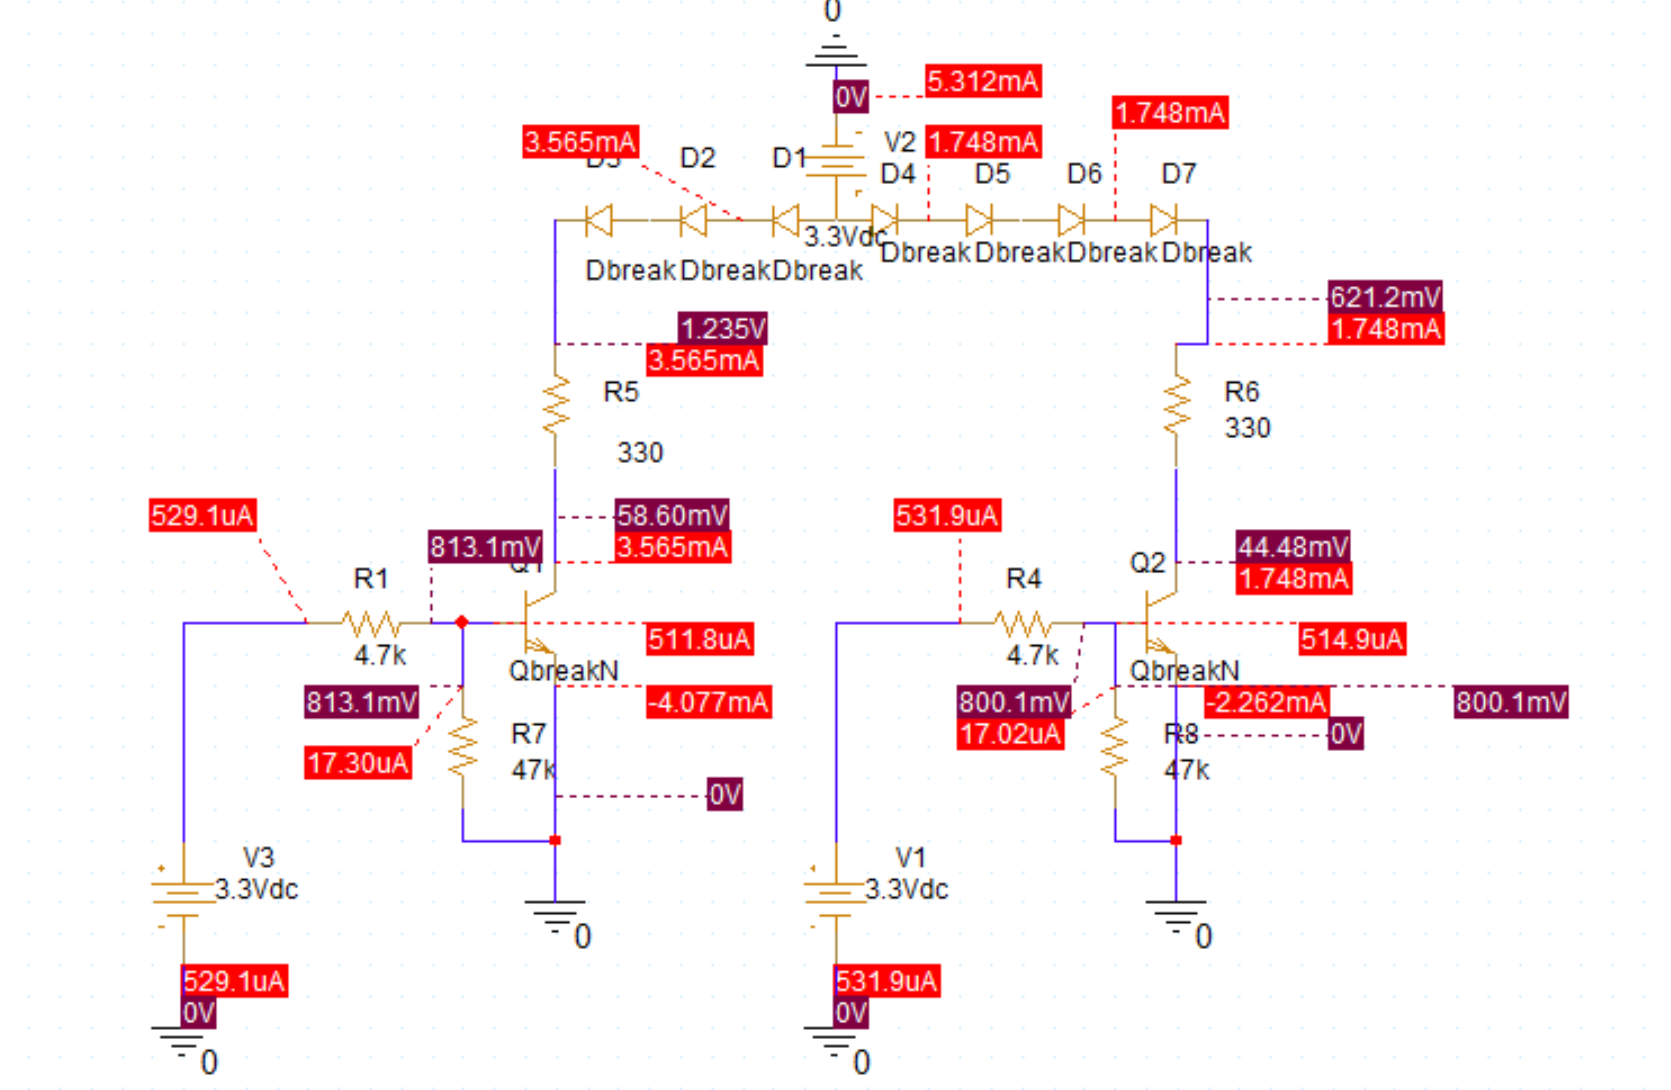
\includegraphics[width=0.95\textwidth]{graphics/section4/f5.png}
    \caption{Simulation led}
\end{figure}


